\documentclass[aspectratio=169,11pt,english]{beamer}

% =========================================================
\usetheme{Berkeley}
\usecolortheme{default}

\definecolor{PythonBlue}{HTML}{306998}
\definecolor{PythonYellow}{HTML}{FFD43B}
\definecolor{DeepNavy}{HTML}{14213D}
\definecolor{SoftWhite}{HTML}{F7F9FC}
\definecolor{CodeGreen}{HTML}{2A9D8F}

\setbeamercolor{structure}{fg=PythonBlue}
\setbeamercolor{palette primary}{bg=DeepNavy,fg=white}
\setbeamercolor{palette secondary}{bg=PythonBlue,fg=white}
\setbeamercolor{palette tertiary}{bg=DeepNavy,fg=white}
\setbeamercolor{palette quaternary}{bg=PythonBlue,fg=white}
\setbeamercolor{title}{fg=white,bg=DeepNavy}
\setbeamercolor{frametitle}{fg=white,bg=DeepNavy}
\setbeamercolor{block title}{fg=white,bg=PythonBlue}
\setbeamercolor{block body}{fg=DeepNavy,bg=SoftWhite}
\setbeamercolor{alerted text}{fg=PythonBlue}
\setbeamercolor{normal text}{fg=DeepNavy,bg=white}
\setbeamercolor{item}{fg=PythonBlue}
\setbeamercolor{section in toc}{fg=PythonBlue}

\setbeamertemplate{navigation symbols}{}
\setbeamertemplate{items}[triangle]
\setbeamertemplate{blocks}[rounded][shadow=false]


\setbeamercovered{invisible}

% =========================================================
% PACKAGES
% =========================================================
\usepackage[T1]{fontenc}
\usepackage[utf8]{inputenc}
\usepackage{babel}
\usepackage{lmodern}
\usepackage{microtype}
\usepackage{graphicx}
\usepackage{booktabs}
\usepackage{mathtools}
\usepackage{amssymb}
\usepackage{xcolor}
\usepackage{listings}
\usepackage{tikz}
\usepackage{hyperref}
\usepackage{listings}
% =========================================================
% PYTHON CODE STYLE
% =========================================================
\lstdefinestyle{pythonstyle}{
	language=Python,
	basicstyle=\ttfamily\small,
	keywordstyle=\color{PythonBlue}\bfseries,
	stringstyle=\color{CodeGreen},
	commentstyle=\color{gray}\itshape,
	numbers=left,
	numberstyle=\tiny\color{gray},
	numbersep=8pt,
	showstringspaces=false,
	breaklines=true,
	frame=single,
	rulecolor=\color{PythonBlue!25},
	backgroundcolor=\color{SoftWhite},
	tabsize=4,
	keepspaces=true,
	columns=fullflexible
}
\lstset{style=pythonstyle}

% =========================================================
% metadata
% =========================================================
\title[CLASS 4.]{Introduction to Programming}
\subtitle{Python Fundamentals}
\author[ ]{Luis Ángel Bustos Ochoa}
\institute{Class 4 }
\date{\today}

% =========================================================
% DOCUMENT
% =========================================================
\begin{document}
	
	% ---------------------------------------------------------
	% FRAME 1 — TITLE PAGE  ---------------------------------------------------------
	{
		\setbeamercolor{background canvas}{bg=DeepNavy}
		\begin{frame}[plain]
			\centering
			\vspace{0.7cm}
			
			{\color{PythonYellow}\rule{0.22\textwidth}{2pt}}
			
			\vspace{0.65cm}
			
			{\color{white}\Huge\bfseries Introduction To Programming\par}
			
			\vspace{0.35cm}
			
			{\color{PythonYellow}\Large Python fundamentals\par}
			
			\vspace{0.8cm}
			
			\begin{tikzpicture}
				\node[
				rounded corners=8pt,
				fill=white,
				text=PythonBlue,
				inner sep=14pt
				] {
					\begin{minipage}{0.58\textwidth}
						\centering
						\ttfamily\Large
						Universidad...
					\end{minipage}
				};
			\end{tikzpicture}
			
			\vfill
			
			{\color{white}\large Luis Ángel Bustos Ochoa\par}
			\vspace{0.15cm}
			{\color{white!75}\normalsize Class 4 \textbar{} Course: \par}
			
			\vspace{0.55cm}
			{\color{PythonYellow}\rule{0.22\textwidth}{2pt}}
			
			\vspace{0.35cm}
			{\color{white!70}\small\insertdate\par}
		\end{frame}
	}	
	% =========================================================
	% SECCIÓN 1
	% =========================================================
%	\section{Roadmap}
	
	% FRAME 2 — WHAT WE WILL LEARN TODAY
	\begin{frame}{Today...}
	%	\framesubtitle{Introduction to the course}
		
		{\large
			\begin{enumerate}
				\item  Translating Yes/No questions into \texttt{True} / \texttt{False}.
								\item \textbf{Comparison Tests}:  \texttt{==}, \texttt{!=}, \texttt{<}, \texttt{>}, \texttt{<=}, \texttt{>=}.
			\item \textbf{Branching Flow}: Routing data through \texttt{if}, \texttt{elif}, and \texttt{else}.
			\end{enumerate}
		}
	\end{frame}
	
	% =========================================================
	% SECCIÓN 2 =========================================================
	\section{Introducing Decisions}
	% FRAME 3 — THE IMPORTANCE OF TWO
	\begin{frame}{Decisions in Python}
	
			\begin{figure}
			\centering
			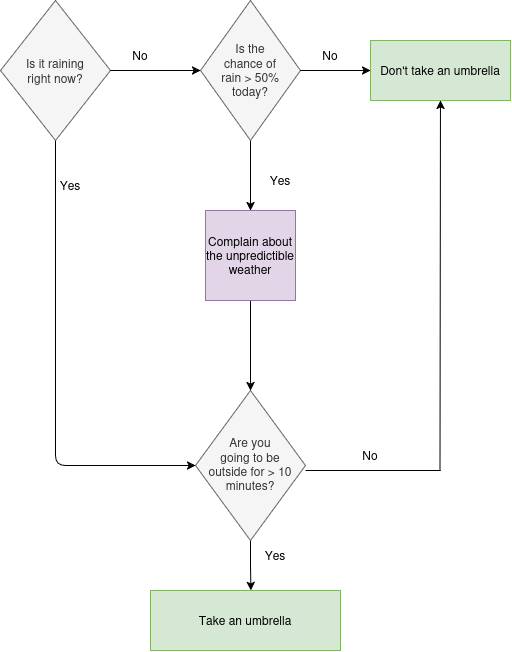
\includegraphics[width=6.9cm, height=6.55cm]{diagram.png}
			
		\end{figure}
	\end{frame}
	\begin{frame}
		\centering
		All yes/no questions can converted to statements that are either true or false. \\
		\pause
		The true/false decision is a python expression that evaluates to a boolean (\textit{Boolean expression}). This kind of statements are called \textbf{conditional statements}
	\end{frame}
	\begin{frame}{Conditional Statements}
		\framesubtitle{introducing "if"}
		\begin{center}
			\textbf{if} statement checks whether the value stored in a variable or the expression is \textit{true or false}	
		\end{center}
		\vspace{0.2cm}
		\pause
		\textbf{Notes:}\\
		\pause
		\underline{don't forget ":"}\\
		\pause
		\underline{In python indentation is very important}\\
		\pause
		\underline{= vs ==}
	\end{frame}
	
	\section{if-elif-else}
\begin{frame}{if vs if-else}
	\framesubtitle{Runs either one or the other, never both}
	
	\begin{columns}[t]
		\begin{column}{0.48\textwidth}
			\centering
			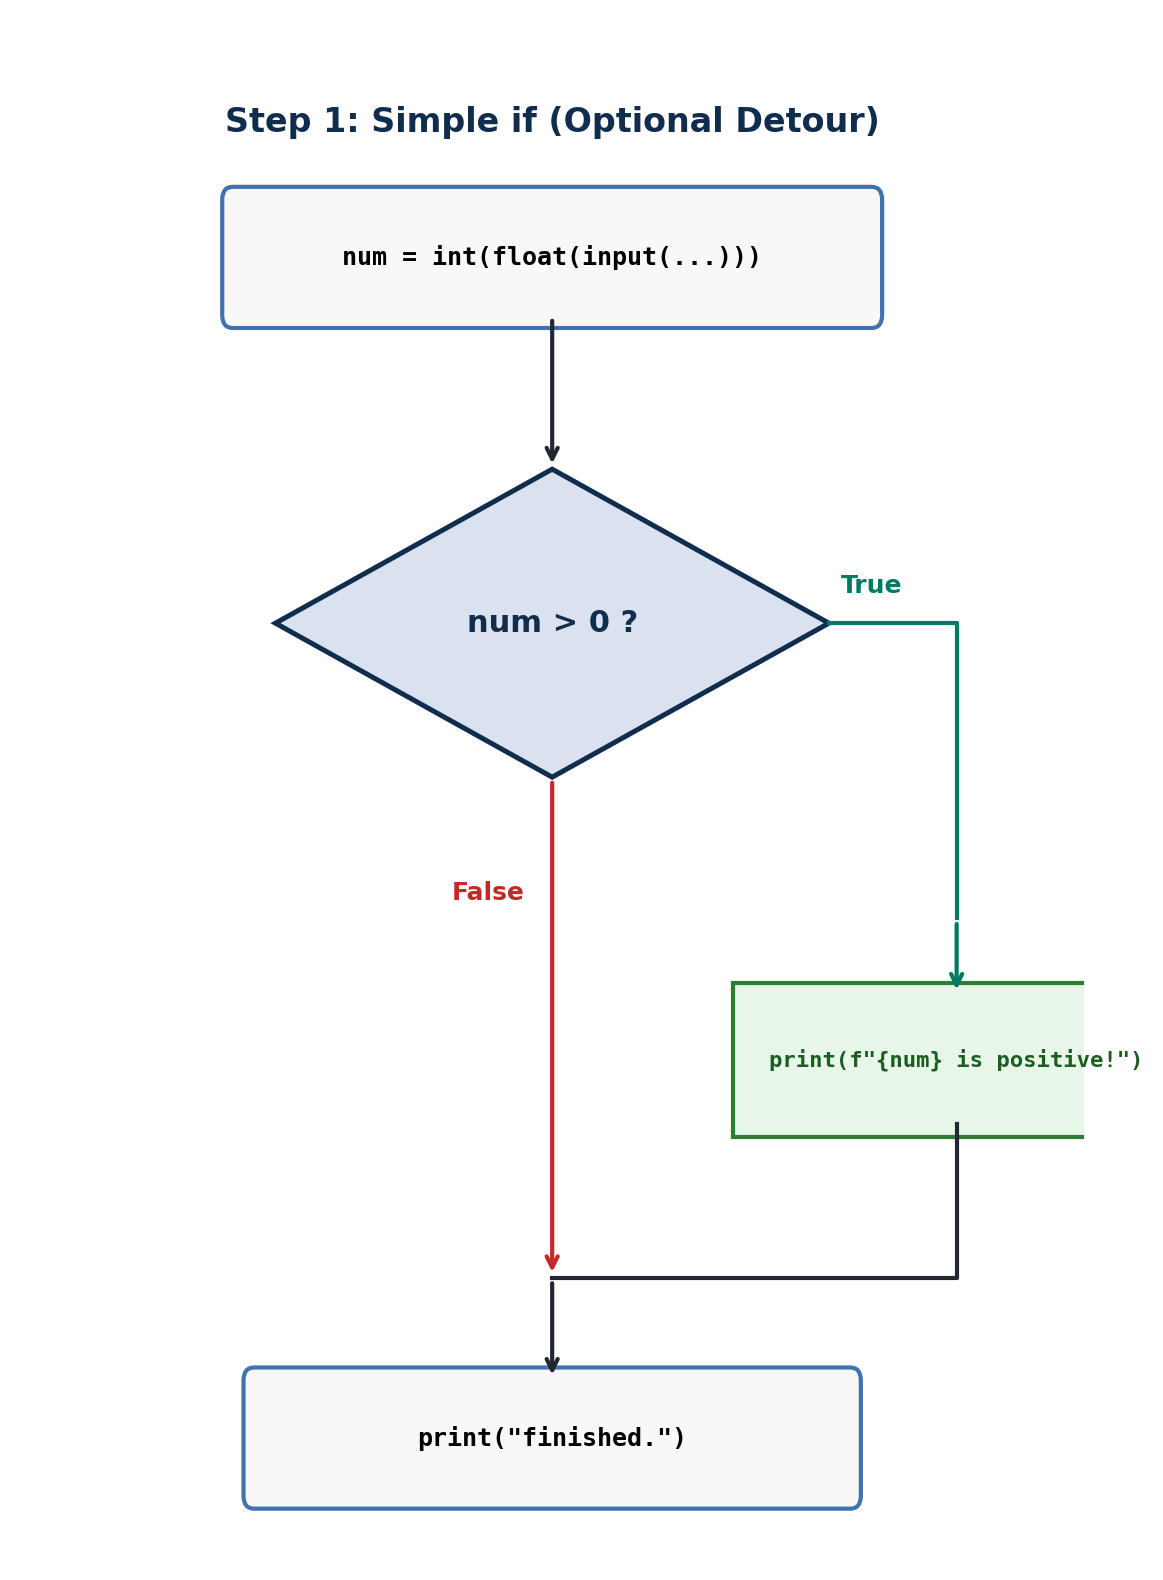
\includegraphics[width=0.85\textwidth]{flowchart_step1_if.png}
		\end{column}
		
		\begin{column}{0.48\textwidth}
			\centering
			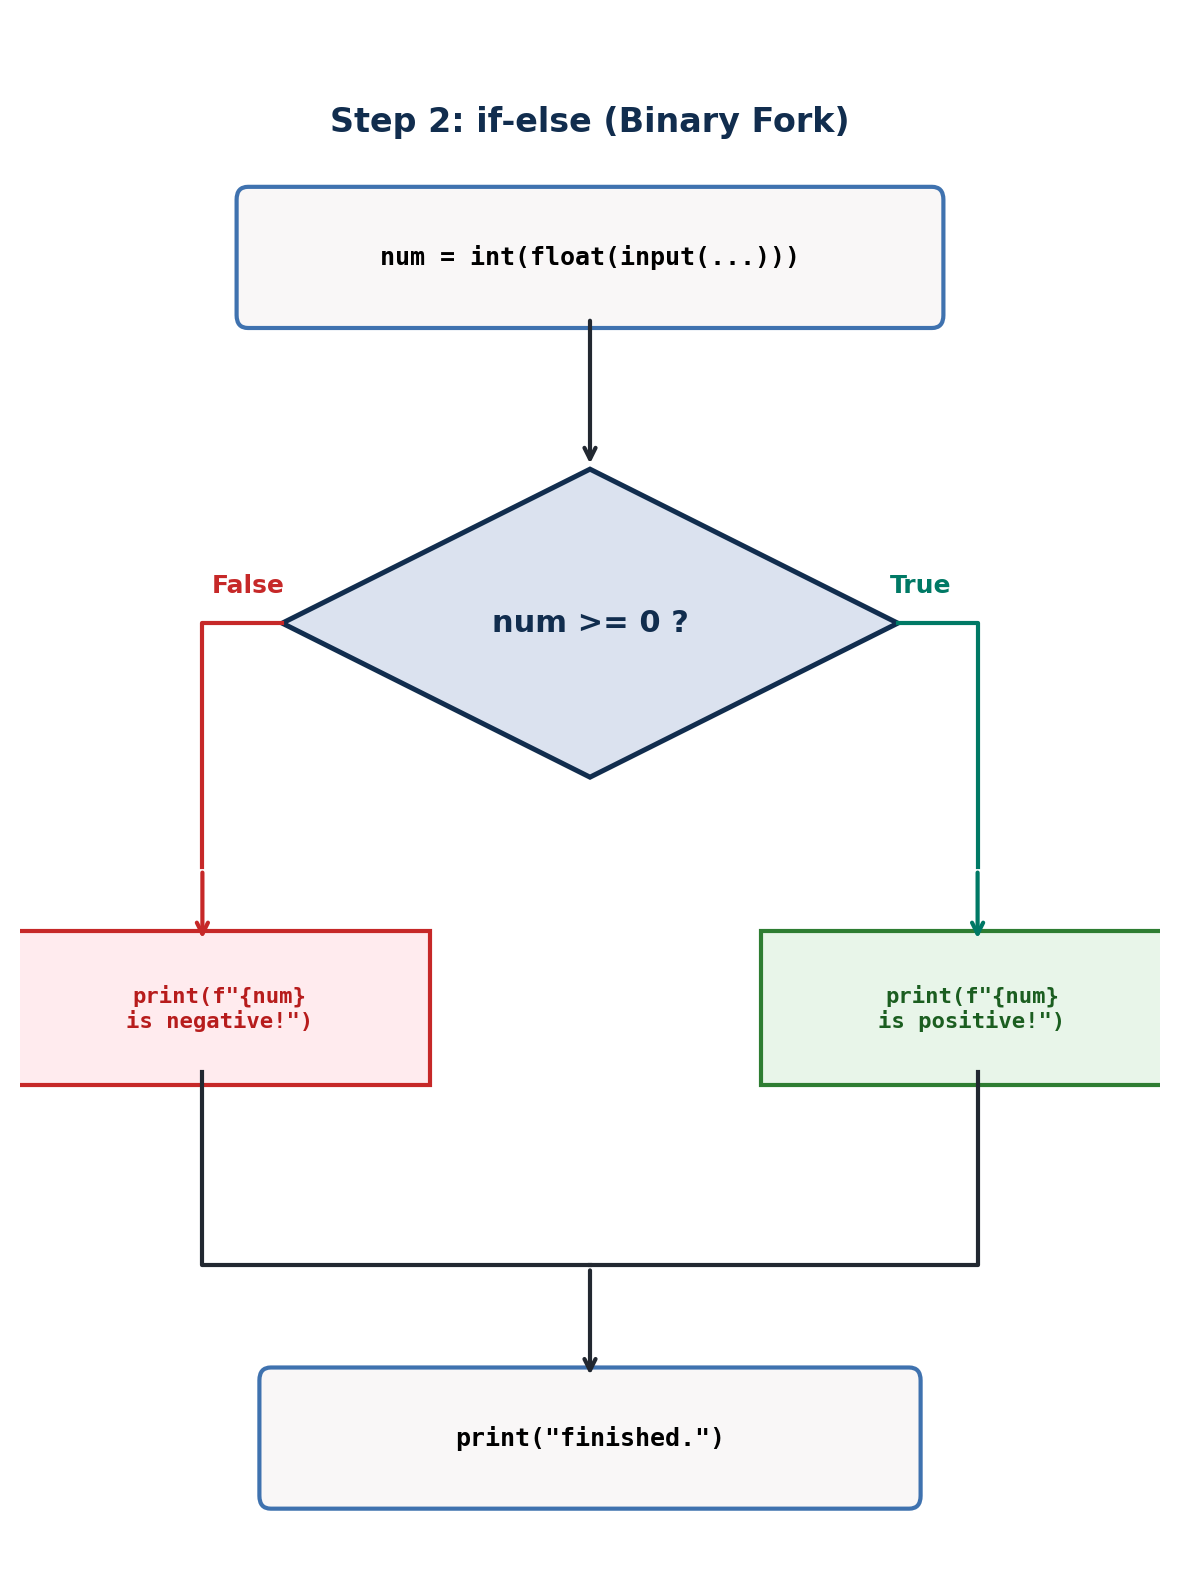
\includegraphics[width=0.85\textwidth]{flowchart_step2_ifelse.png}
		\end{column}
	\end{columns}

	\end{frame}
		\begin{frame}{Elif}
		\centering
		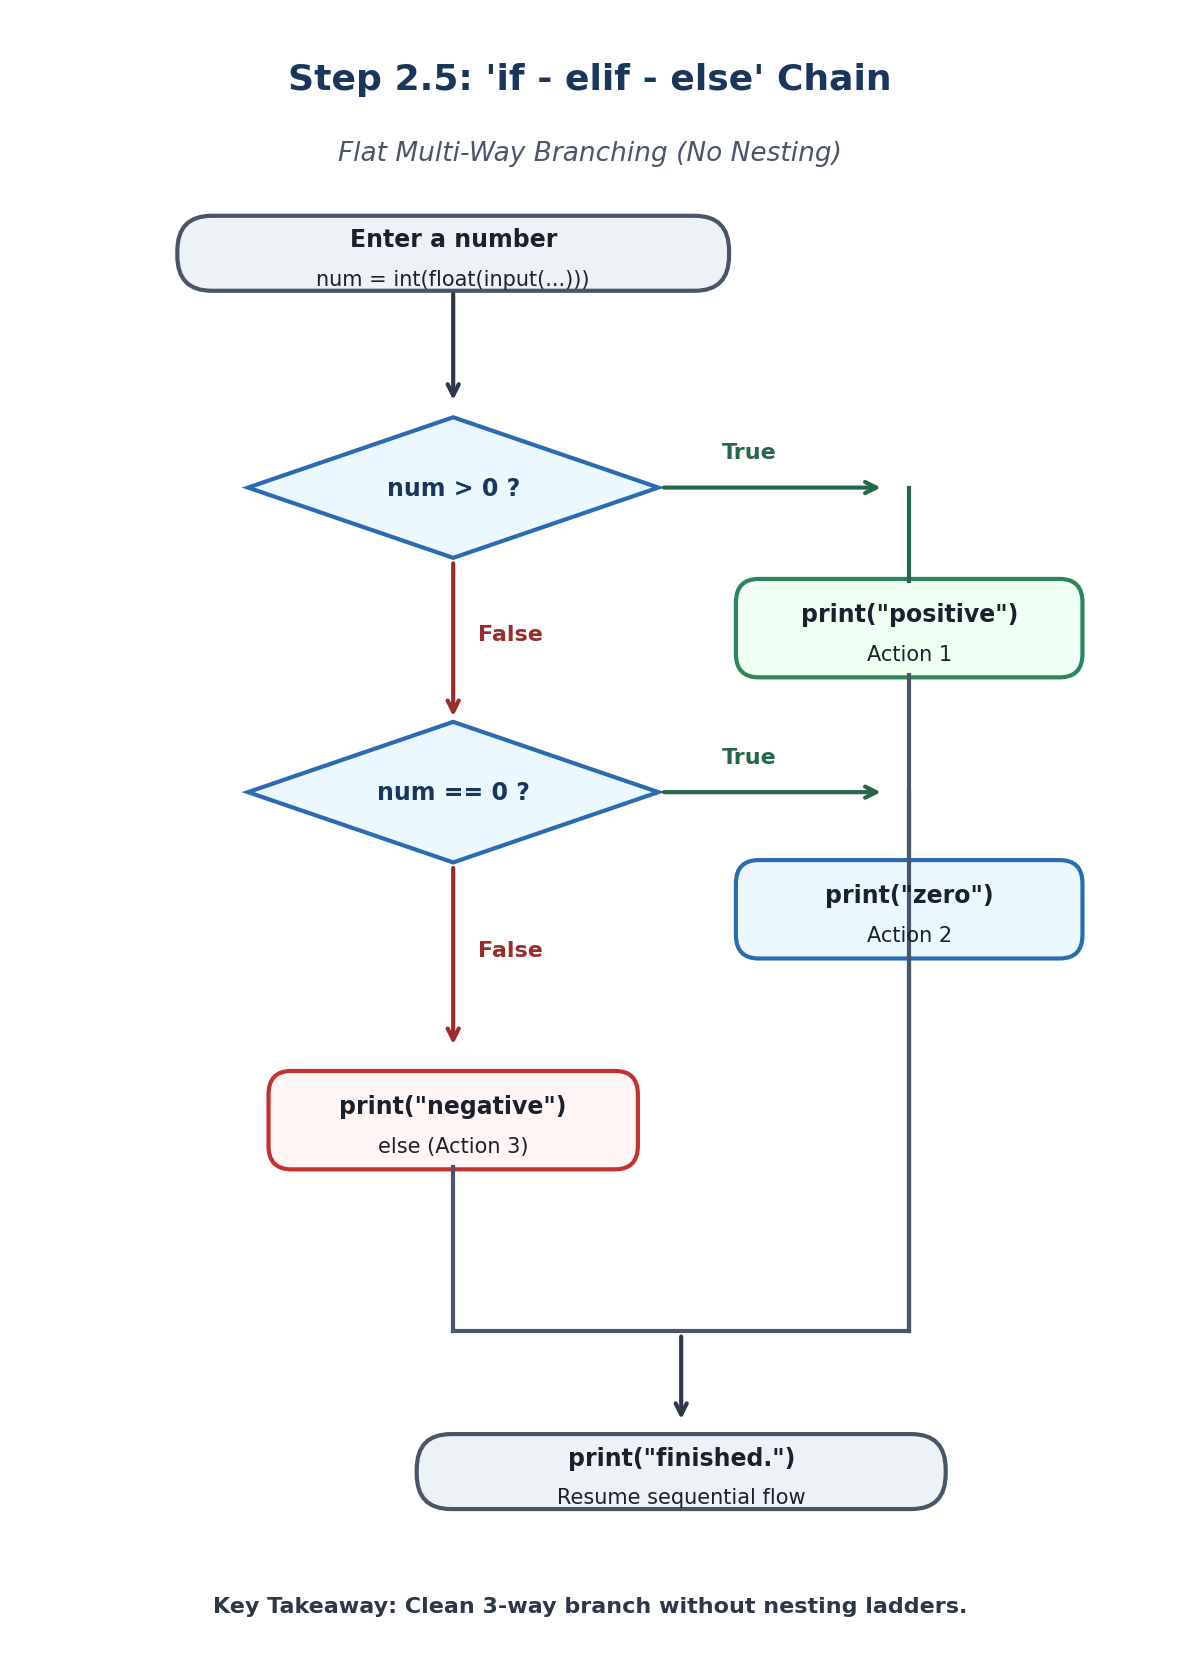
\includegraphics[width=0.38\textwidth]{flowchart_step2_5_elif.png}
	\end{frame}

	\begin{frame}{Introduction to Nested code}
	
		
		 \centering
				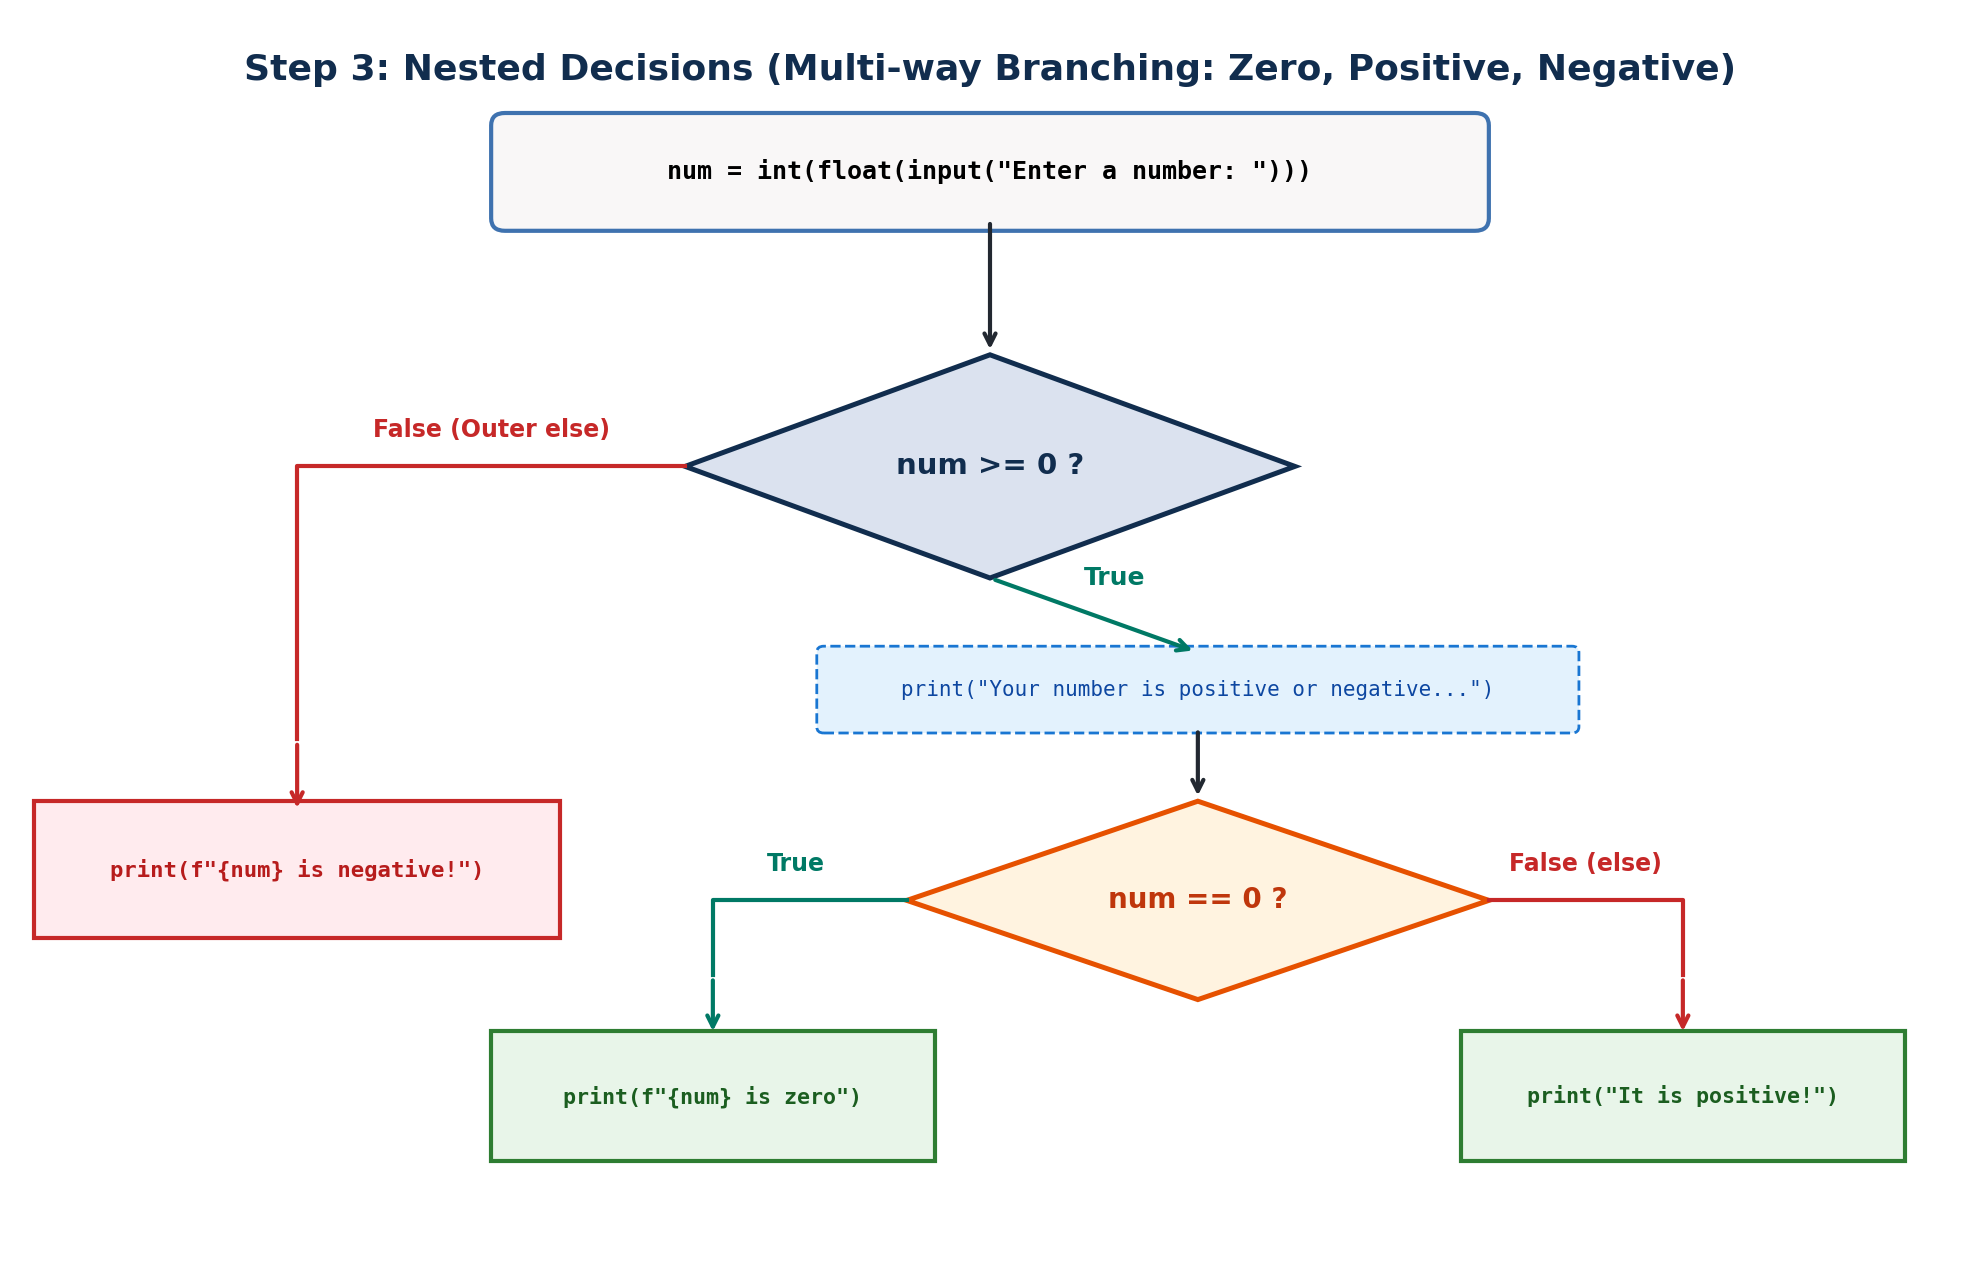
\includegraphics[width=0.95\textwidth]{flowchart_step3_nested.png}
		
			
		
	\end{frame}
	\begin{frame}[fragile]{Exercise: Nested Trap vs. Sequential Flow}
		\framesubtitle{Predict the exact console output for each input value}
		
		\begin{columns}[t]
			\begin{column}{0.48\textwidth}
				\setbeamercolor{block title}{use=bloquetitder, bg=bloquetitder.bg, fg=bloquetitder.fg}
				\setbeamercolor{block body}{use=bloqueder, bg=bloqueder.bg, fg=bloqueder.fg}
				\begin{block}{ Nested (Deep Indent)}
					\begin{semiverbatim}\fontsize{7.5pt}{9pt}\selectfont
						score = int(input())
						if score >= 60:
						----print("Pass:")
						----if score >= 90:
						------print("Honors!")
						----else:
						------print("Regular")
						else:
						----print("Fail")
					\end{semiverbatim}
				\end{block}
			\end{column}
			
			\begin{column}{0.48\textwidth}
				\setbeamercolor{block title}{use=bloquetitizq, bg=bloquetitizq.bg, fg=bloquetitizq.fg}
				\setbeamercolor{block body}{use=bloqueizq, bg=bloqueizq.bg, fg=bloqueizq.fg}
				\begin{block}{Flat Sequential (\texttt{elif})}
					\begin{semiverbatim}\fontsize{7.5pt}{9pt}\selectfont
						score = int(input())
						if score >= 90:
						print("Honors!")
						elif score >= 60:
						print("Pass")
						else:
						print("Fail")
					\end{semiverbatim}
				\end{block}
			\end{column}
		\end{columns}
		
		\vspace{0.15cm}
		\centering
		\renewcommand{\arraystretch}{1.2}
		\begin{tabular}{|c|p{4.7cm}|p{4.7cm}|}
			\hline
			\textbf{Input (\texttt{score})} & \textbf{Option A Output} & \textbf{Option B Output} \\ \hline
			\texttt{95}  & \textit{Predict...} & \textit{Predict...} \\ \hline
			\texttt{80}  & \textit{Predict...} & \textit{Predict...} \\ \hline
			\texttt{50}  & \textit{Predict...} & \textit{Predict...} \\ \hline
		\end{tabular}
	\end{frame}
	\subsection{Combining conditions}
	\begin{frame}{ This or that or some other thing}
		\framesubtitle{Truth Values}
		\begin{columns}[t]
			\begin{column}{0.30\textwidth}
				\setbeamercolor{block title}{use=bloquetitder, bg=bloquetitder.bg, fg=bloquetitder.fg}
				\setbeamercolor{block body}{use=bloqueder, bg=bloqueder.bg, fg=bloqueder.fg}
				\begin{block}{\texttt{not A} (Invert)}
					\centering
					\renewcommand{\arraystretch}{1.1}
					\begin{tabular}{|c|c|}
						\hline
						\textbf{A} & \textbf{not A} \\ \hline
						\texttt{True}  & \texttt{False} \\ \hline
						\texttt{False} & \texttt{True}  \\ \hline
					\end{tabular}
					\vspace{0.15cm}
					\footnotesize Reverses the truth value.
				\end{block}
			\end{column}
			
			\begin{column}{0.34\textwidth}
				\setbeamercolor{block title}{use=bloquetitizq, bg=bloquetitizq.bg, fg=bloquetitizq.fg}
				\setbeamercolor{block body}{use=bloqueizq, bg=bloqueizq.bg, fg=bloqueizq.fg}
				\begin{block}{\texttt{A and B} (Strict)}
					\centering
					\renewcommand{\arraystretch}{1.1}
					\begin{tabular}{|c|c|c|}
						\hline
						\textbf{A} & \textbf{B} & \textbf{Result} \\ \hline
						\texttt{T} & \texttt{T} & \textbf{\texttt{True}} \\ \hline
						\texttt{T} & \texttt{F} & \texttt{False} \\ \hline
						\texttt{F} & \texttt{T} & \texttt{False} \\ \hline
						\texttt{F} & \texttt{F} & \texttt{False} \\ \hline
					\end{tabular}
					\vspace{0.15cm}
%					\footnotesize \textbf{Both} must be True.
				\end{block}
			\end{column}
			
			\begin{column}{0.34\textwidth}
				\setbeamercolor{block title}{use=bloquetitizq, bg=bloquetitizq.bg, fg=bloquetitizq.fg}
				\setbeamercolor{block body}{use=bloqueizq, bg=bloqueizq.bg, fg=bloqueizq.fg}
				\begin{block}{\texttt{A or B} (Flexible)}
					\centering
					\renewcommand{\arraystretch}{1.1}
					\begin{tabular}{|c|c|c|}
						\hline
						\textbf{A} & \textbf{B} & \textbf{Result} \\ \hline
						\texttt{T} & \texttt{T} & \textbf{\texttt{True}} \\ \hline
						\texttt{T} & \texttt{F} & \textbf{\texttt{True}} \\ \hline
						\texttt{F} & \texttt{T} & \textbf{\texttt{True}} \\ \hline
						\texttt{F} & \texttt{F} & \texttt{False} \\ \hline
					\end{tabular}
					\vspace{0.15cm}
%					\footnotesize \textbf{At least one} is True.
				\end{block}
			\end{column}
		\end{columns}
	\end{frame}
	\begin{frame}{Order of Operations (Precedence)}

		
		\centering
		\renewcommand{\arraystretch}{1.2}
		\begin{tabular}{|c|l|l|}
			\hline
			\textbf{Priority} & \textbf{Operator Type} & \textbf{Examples} \\ \hline
			\textbf{1 (Highest)} & Parentheses & \texttt{(a or b)} \\ \hline
			\textbf{2} & Arithmetic (Math) & \texttt{**}, \texttt{*}, \texttt{/}, \texttt{+}, \texttt{-} \\ \hline
			\textbf{3} & Relational Tests & \texttt{==}, \texttt{!=}, \texttt{<}, \texttt{>}, \texttt{<=}, \texttt{>=} \\ \hline
			\textbf{4} & Boolean NOT & \texttt{not} \\ \hline
			\textbf{5} & Boolean AND & \texttt{and} \\ \hline
			\textbf{6 (Lowest)} & Boolean OR & \texttt{or} \\ \hline
		\end{tabular}
		
		\vspace{0.3cm}
		\begin{columns}[t]
			\begin{column}{0.95\textwidth}
				\setbeamercolor{block title}{use=bloquetitder, bg=bloquetitder.bg, fg=bloquetitder.fg}
				\setbeamercolor{block body}{use=bloqueder, bg=bloqueder.bg, fg=bloqueder.fg}
				\begin{block}{Good practice:}
					\footnotesize When in doubt, \textbf{use parentheses \texttt{()}} to make your logic explicit and avoid unexpected bugs.
				\end{block}
			\end{column}
		\end{columns}
	\end{frame}
\end{document}